\documentclass{book}
\usepackage{hyperref}
\usepackage{url}
\usepackage{amsmath}
%%\VignetteIndexEntry{Using the Devore6 package}
%%\VignetteDepends{Devore6}
\usepackage{/usr/local/lib/R/share/texmf/Sweave}
\begin{document}

\setkeys{Gin}{width=\textwidth}
\title{Using the Devore6 package with R}
\author{Douglas Bates\\Department of Statistics\\
  University of Wisconsin-Madison}
\date{}
\maketitle

\tableofcontents

\setcounter{chapter}{-1}
\chapter{Preliminaries}

This document describes the use of the statistical package R as
computing support in an introductory statistics course based on the text
\emph{Probability and Statistics for Engineering and the Sciences (6th
edition)} by Jay Devore (Duxbury, 2004).  We demonstrate how R can be
used to reproduce the results in many of the examples in the text.

One of the desirable features of this text is the number of examples
and exercises based on real data sets the Prof.{} Devore has culled
from the engineering literature.  As they are real data, some of the
data sets are large and have a complex structure.  Although it is not
difficult to enter these data into a computer package like R, the
process is tedious and error-prone.  Furthermore, it is not much of a
learning experience.

We have provided copies of the data sets for the examples and the
exercises in a ``package'', named \texttt{Devore6}, that can be used
with R.  This document is also part of the \texttt{Devore6} package.

You may wish to try some of the examples in this section as you are
reading it.  We assume that you have both R and the Devore6
package for R installed.  (See Appendix~\ref{app:Installing} for
instructions if you need to do this first.)

\subsection*{Calculating a median}
\label{prelim:xmp0114}

Suppose that we wish to reproduce the calculation of the median of the
data on transferrin receptor concentration shown in Example 1.14
(p.~31 of the text).  As there are only 12 concentrations, we could
enter the data by hand.  Start R and type
\begin{Schunk}
\begin{Sinput}
> conc = c(15.2, 9.3, 7.6, 11.9, 10.4, 9.7, 20.4, 9.4, 11.5, 
+     16.2, 9.4, 8.3)
> str(conc)
\end{Sinput}
\begin{Soutput}
 num [1:12] 15.2 9.3 7.6 11.9 10.4 9.7 20.4 9.4 11.5 16.2 ...
\end{Soutput}
\begin{Sinput}
> median(conc)
\end{Sinput}
\begin{Soutput}
[1] 10.05
\end{Soutput}
\end{Schunk}

The first line assigns the 12 data values as a numeric vector to the
name \texttt{conc}, a short form of ``concentration''.  The function
named \texttt{"c"} concatenates a series of data values into a vector
that can be assigned a name.

In the next line the \texttt{"str"} function is used to examine the
structure of the object named \texttt{"conc"}.  The output shows that
this is a numeric vector of length 12 and displays the first several
data values so you can check them against the data in the text.

Finally the \texttt{"median"} function, applied to the \texttt{conc}
vector returns the median.

\subsection*{Using the Devore6 package}
\label{sec:UsingDevore6}

Entering the data, as shown above, is suitable for small data sets.
An alternative and preferred way to access the data, especially for
the larger data sets, is to use the \texttt{Devore6} package and load
the data set.  The data set for Example 1.14 is called
\texttt{xmp01.14}.  In general, data sets for examples in the text are
named \texttt{xmp}\textit{cc.nn}, where \textit{cc} is the two-digit
chapter number and \textit{nn} is the two-digit example number.
Data sets for exercises are named \texttt{ex}\textit{cc.nn}.  (Single
digit chapter or example numbers have a \texttt{0} prepended as in
\texttt{xmp01.14} so that the names sort in the correct order.)

You must attach the \texttt{Devore6} package every time you start R if
you are to have access to the data sets from the textbook like this.

To attach the package to an R session use
\begin{Schunk}
\begin{Sinput}
> library(Devore6)
\end{Sinput}
\end{Schunk}
after starting R or select \texttt{Packages -> Load package ->
  Devore6} from the menu bar.  (If this produces an error see
Appendix~\ref{app:Installing} for instructions on installing the
\texttt{Devore6} package.)

After attaching the package, you can load a data set with
\begin{Schunk}
\begin{Sinput}
> data(xmp01.14)
> str(xmp01.14)
\end{Sinput}
\begin{Soutput}
`data.frame':	12 obs. of  1 variable:
 $ concentration: num  15.2 9.3 7.6 11.9 10.4 9.7 20.4 9.4 11.5 16.2 ...
\end{Soutput}
\end{Schunk}

The first line loads the data set into the current R session.  The
second line provides a description of the structure of the data set.
It is a good practice always to use \texttt{str} on the data set after
loading it.

\subsection*{Form of the data sets}
\label{sec:Form}

The data set \texttt{xmp01.14} is not a single vector like
\texttt{conc}.  It is a data table (called a ``data frame'' in R) with
one column and 12 rows.  All the data sets in the \texttt{Devore6}
package are data frames.

The output from \texttt{str} indicates that the name of the first
column is \texttt{concentration}.  To calculate the median we must
give both the name of the data frame and the name of the column.  We
can do this in three ways, as described in
Appendix~\ref{app:accessCols}.  We will focus on just one of these
ways, which is to use the \texttt{"with"} function.
\begin{Schunk}
\begin{Sinput}
> with(xmp01.14, median(concentration))
\end{Sinput}
\begin{Soutput}
[1] 10.05
\end{Soutput}
\end{Schunk}

The \texttt{with} function indicates which data set should be used to
gain access to the column (or ``variable'') called \texttt{concentration}.

\subsection*{Summary}
\label{sec:prelim:summary}

To recap:
\begin{enumerate}
\item You should have R installed on a computer and the
  \texttt{Devore6} package for R installed.  (See
  Appendix~\ref{app:Installing} for instructions if you need to do
  this.)

\item At the beginning of each session use
\begin{Schunk}
\begin{Sinput}
> library(Devore6)
\end{Sinput}
\end{Schunk}
to allow access to the data sets from the package.
\item To load the data for a specific example or a specific exercise
  use a name of the form \texttt{xmp}\textit{cc.nn} or
  \texttt{ex}\textit{cc.nn} to \texttt{data()} then check the
  structure with \texttt{str()}.
\begin{Schunk}
\begin{Sinput}
> data(xmp01.14)
> str(xmp01.14)
\end{Sinput}
\end{Schunk}
\end{enumerate}
In the remainder of this document we will not show these steps
explicitly.

The R functions we have mentioned are shown in Table~\ref{tab:general}.  See also Appendix~\ref{app:help}.

\begin{table}[htbp]
  \centering
  \begin{tabular}[]{l l}
    Function & Purpose \\\hline
    q()         & quit R\\
    help(name)  & display help on an object (function or data set)\\
    help.search(``topic'')& search for functions related to a topic\\
    library(name)  & Make data sets from a package available for loading\\
    data(name)     & Load a data set \\
    str(name)      & Display a brief description of the structure \\
    with(dataset,$\dots$)  & Use the variables in a data set \\
    \hline
  \end{tabular}
  \caption{R functions for general use}
  \label{tab:general}
\end{table}


\chapter{Overview and Descriptive Statistics}
\label{ch:overview}

We will follow the same sequence of topics and chapter headings as in
the text and will begin each chapter with a table of R functions that
are used in the chapter.

Table~\ref{tab:ch1} lists functions used in chapter 1.
\begin{table}[htbp]
  \centering
  \begin{tabular}{l l}
    \multicolumn{1}{c}{\textbf{Function}} &
    \multicolumn{1}{c}{\textbf{Description}} \\\hline
    stem(x)   & stem-and-leaf display\\
    hist(x)   & histogram\\
    boxplot(x)& boxplot\\
    mean(x)   & mean (i.e. average) value of x\\
    median(x) & median\\
    var(x)    & sample variance\\
    sd(x)     & sample standard deviation\\
    log(x)    & natural logarithm (works on entire vectors)\\
    log(x, 10)& common (base 10) logarithm\\
    sqrt(x)   & square root\\
    \verb+x^(1/3)+  & cube root\\
    \hline
  \end{tabular}
  \caption{R functions used with chapter 1}
  \label{tab:ch1}
\end{table}

\section{Example 1.1}
\label{sec:xmp01.01}

Example 1.1 (p.~4) lists the ambient temperatures ($^\circ$F) for each
test firing or actual launch of the space shuttle prior to the
\emph{Challenger} tradgedy in 1986.  In Figure 1.1 (p.~5) these data
are displayed as a stem-and-leaf plot and as a histogram.  There are
36 data values.

A stem-and-leaf plot similar to that in Figure 1.1 (p.~5) can be produced with
\begin{Schunk}
\begin{Sinput}
> with(xmp01.01, stem(temp))
\end{Sinput}
\begin{Soutput}
  The decimal point is 1 digit(s) to the right of the |

  3 | 1
  4 | 059
  5 | 23788
  6 | 01136777789
  7 | 000023556689
  8 | 0134
\end{Soutput}
\end{Schunk}
(Remember that first you must attach the \texttt{Devore6} package,
load the \texttt{xmp01.01} data set and check its structure.  We do
not show those steps here.)

The \texttt{hist} function produces a histogram.
\begin{center}
\begin{Schunk}
\begin{Sinput}
> with(xmp01.01, hist(temp))
\end{Sinput}
\end{Schunk}
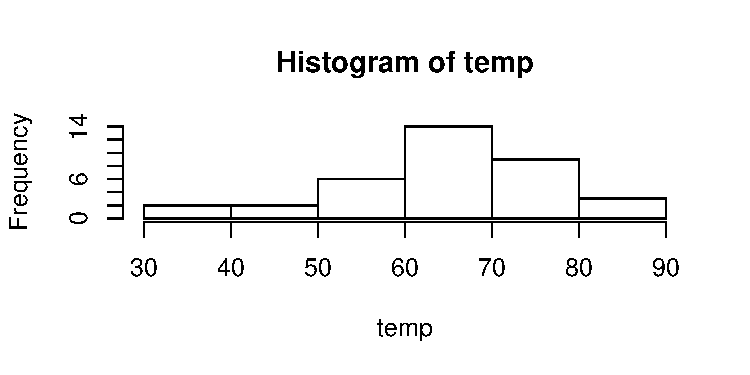
\includegraphics{Devore6-009}
\end{center}

The stem-and-leaf plot and the histogram shown here are not exactly
the same as those shown in Figure 1.1 (p.~5).  In
section~\ref{sec:ch1enhance} we show how optional arguments to
\texttt{stem} and to \texttt{hist} could be used to produce displays
similar to those in the text.

\section{Example 1.5}
\label{sec:xmp01.05}

The data in example 1.3 (p.~12), on the percentage of undergraduate
students who are binge drinkers at 140 different campuses, are
presented as a stem-and-leaf display in Figure 1.4 (p.~12).
\begin{Schunk}
\begin{Sinput}
> with(xmp01.05, stem(bingePct))
\end{Sinput}
\begin{Soutput}
  The decimal point is 1 digit(s) to the right of the |

  0 | 4
  0 | 
  1 | 134
  1 | 5678889
  2 | 12234
  2 | 56666777889999
  3 | 0112233344
  3 | 555666677777888899999
  4 | 11122222334444
  4 | 5566666677788888999
  5 | 001112222334
  5 | 55666667777888899
  6 | 011112444
  6 | 55666778
\end{Soutput}
\begin{Sinput}
> with(xmp01.05, stem(bingePct, scale = 0.5))
\end{Sinput}
\begin{Soutput}
  The decimal point is 1 digit(s) to the right of the |

  0 | 4
  1 | 1345678889
  2 | 1223456666777889999
  3 | 0112233344555666677777888899999
  4 | 111222223344445566666677788888999
  5 | 00111222233455666667777888899
  6 | 01111244455666778
\end{Soutput}
\end{Schunk}

The first stem-and-leaf display is more spread out than the one in
Figure~1.4 (p.~12).  In the second call to \texttt{stem} we use the
optional argument \texttt{scale} to shrink the scale by a factor of
$\frac{1}{2}$ so the resulting display is similar to that in
Figure~1.4.


\section{Example 1.6}
\label{sec:xmp01.06}

As in Example~1.5 a stem-and-leaf display is created, this time from
data on yardages of golf courses as given in \emph{Golf Magazine}.
\begin{Schunk}
\begin{Sinput}
> with(xmp01.06, stem(yardage))
\end{Sinput}
\begin{Soutput}
  The decimal point is 2 digit(s) to the right of the |

  64 | 3467
  65 | 1338
  66 | 119
  67 | 015779
  68 | 05779
  69 | 0034
  70 | 112455
  71 | 113777
  72 | 18
\end{Soutput}
\end{Schunk}


\section{Examples 1.7 and 1.8}
\label{sec:xmp01.07}

Example~1.7 describes the \emph{time-series plot} in Figure~1.6
(p.~14) of quarterly beer consumption.  These data are not available
so we show how a time-series plot of the shuttle launch temperatures
from Example~1.1 could be created.



\begin{center}
\begin{Schunk}
\begin{Sinput}
> with(xmp01.01, plot(temp, type = "b"))
\end{Sinput}
\end{Schunk}
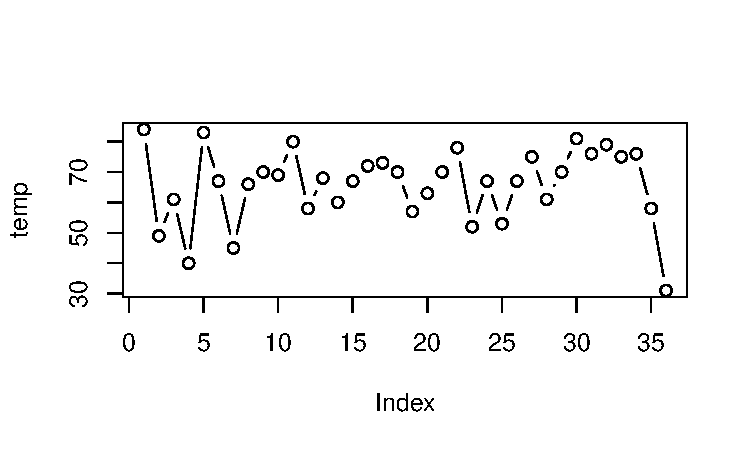
\includegraphics{Devore6-xmp0107}
\end{center}%$
The optional argument \texttt{type="b"} to the \texttt{plot} function
indicates that both the points and the connecting lines should be drawn on
the plot.

There is no easy way to use R to produce the dotplot shown in
Figure~1.7 (p.~14) for Example~1.8.


\section{Example 1.10}
\label{sec:xmp01.10}

A histogram such as shown in Figure~1.9 (p.~19) is produced by the
\texttt{hist} function.
\begin{center}
\begin{Schunk}
\begin{Sinput}
> with(xmp01.10, hist(consump))
\end{Sinput}
\end{Schunk}
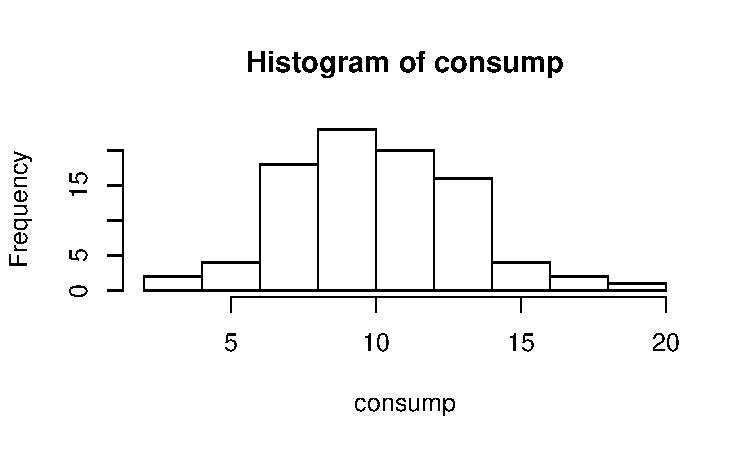
\includegraphics{Devore6-xmp0110}
\end{center}
The vertical axis on this histogram is frequency.  For a vertical axis
on the scale of density (relative frequency divided by bin width) use
the optional argument \texttt{freq = FALSE}.


\section{Example 1.11}
\label{sec:xmp01.11}

Figure~1.11 (p.~20) shows an example of a histogram with unequal bin
widths.  The optional argument \texttt{breaks} to the \texttt{hist}
function is used to set the breakpoints for the bins.  When unequal
bin widths are used, the vertical axis switches to the density scale.
\begin{center}
\begin{Schunk}
\begin{Sinput}
> with(xmp01.11, hist(strength, breaks = c(2, 4, 6, 8, 12, 
+     20, 30)))
\end{Sinput}
\end{Schunk}
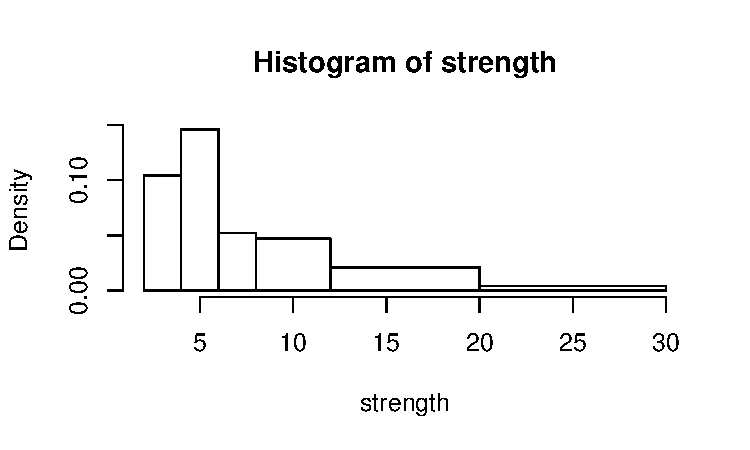
\includegraphics{Devore6-xmp0111}
\end{center}
The \texttt{breaks} argument is a vector created by concatenating
several numbers with the \texttt{c} function.


\section{Example 1.12}
\label{sec:xmp01.12}

Figure~1.13 (p.~22) shows a barplot for the motorcycle ownership
data.  As this data set is not available in the \texttt{Devore6}
package, we create the vector of
frequencies, assign names to the frequencies, and then use
\texttt{barplot} to produce the plot
\begin{Schunk}
\begin{Sinput}
> cycles = c(41, 27, 20, 18, 3, 11)
> names(cycles) = c("Honda", "Yamaha", "Kawasaki", "Harley", 
+     "BMW", "other")
> barplot(cycles)
\end{Sinput}
\end{Schunk}
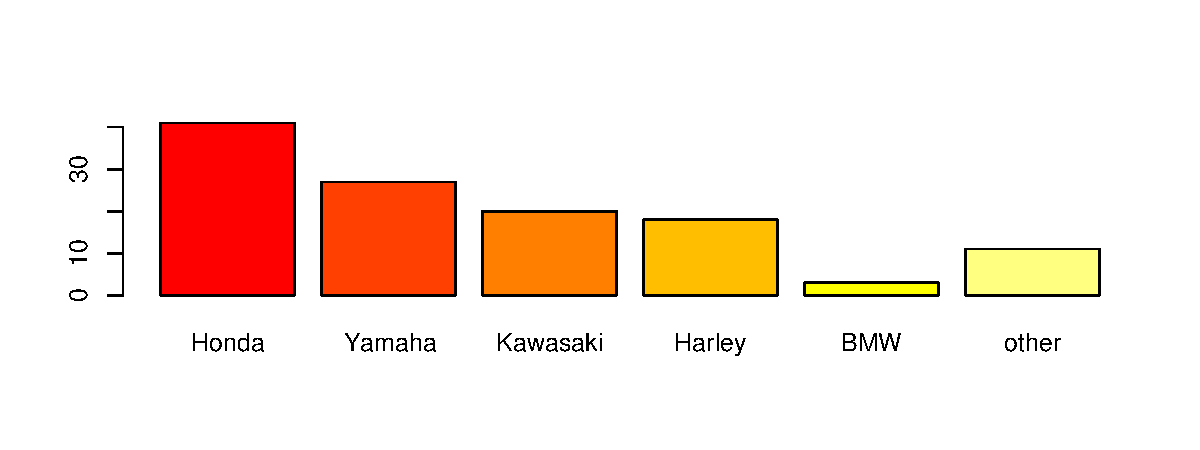
\includegraphics{Devore6-xmp0112}


\section{Examples 1.13 and 1.14}
\label{sec:xmp01.13}

Numeric measures of location are calculated with the functions
\texttt{mean} and \texttt{median}.  Another useful summary function is
\texttt{sum}.  A brief summary, including the mean, the median, the
quartiles, the maximum and minimum is returned by \texttt{summary}.
\begin{Schunk}
\begin{Sinput}
> with(xmp01.13, mean(crackLength))
\end{Sinput}
\begin{Soutput}
[1] 21.18095
\end{Soutput}
\begin{Sinput}
> with(xmp01.13, sum(crackLength))
\end{Sinput}
\begin{Soutput}
[1] 444.8
\end{Soutput}
\begin{Sinput}
> with(xmp01.14, median(concentration))
\end{Sinput}
\begin{Soutput}
[1] 10.05
\end{Soutput}
\begin{Sinput}
> with(xmp01.13, summary(crackLength))
\end{Sinput}
\begin{Soutput}
   Min. 1st Qu.  Median    Mean 3rd Qu.    Max. 
   8.90   14.00   21.20   21.18   25.80   45.00 
\end{Soutput}
\begin{Sinput}
> with(xmp01.14, summary(concentration))
\end{Sinput}
\begin{Soutput}
   Min. 1st Qu.  Median    Mean 3rd Qu.    Max. 
  7.600   9.375  10.050  11.610  12.730  20.400 
\end{Soutput}
\end{Schunk}

\section{Example 1.15}
\label{sec:xmp01.15}

The trimmed mean, described in Example~1.15 (p.~32) is obtained by using
the optional \texttt{trim} argument to \texttt{mean}.
\begin{Schunk}
\begin{Sinput}
> with(xmp01.15, summary(lifetime))
\end{Sinput}
\begin{Soutput}
   Min. 1st Qu.  Median    Mean 3rd Qu.    Max. 
  612.0   894.3  1010.0   965.0  1086.0  1201.0 
\end{Soutput}
\begin{Sinput}
> with(xmp01.15, mean(lifetime, trim = 0.1))
\end{Sinput}
\begin{Soutput}
[1] 979.125
\end{Soutput}
\end{Schunk}


\section{Example 1.16}
\label{sec:xmp01.16}

Functions \texttt{var} and \texttt{sd} provide the sample variance and
sample standard deviation, respectively.  The ``computing formula''
described on p.~39 is not used by these functions because that formula
can have poor numerical properties.
\begin{Schunk}
\begin{Sinput}
> with(xmp01.16, var(Strength))
\end{Sinput}
\begin{Soutput}
[1] 1.193580
\end{Soutput}
\begin{Sinput}
> with(xmp01.16, sd(Strength))
\end{Sinput}
\begin{Soutput}
[1] 1.092511
\end{Soutput}
\end{Schunk}


\section{Examples 1.18}
\label{sec:xmp01.18}

Function \texttt{boxplot} provides the boxplot.  By default a vertical
boxplot is constructed.  Use the optional argument
\texttt{horizontal=TRUE} to get a horizontal boxplot
\begin{center}
\begin{Schunk}
\begin{Sinput}
> with(xmp01.18, boxplot(depth, horizontal = TRUE))
\end{Sinput}
\end{Schunk}
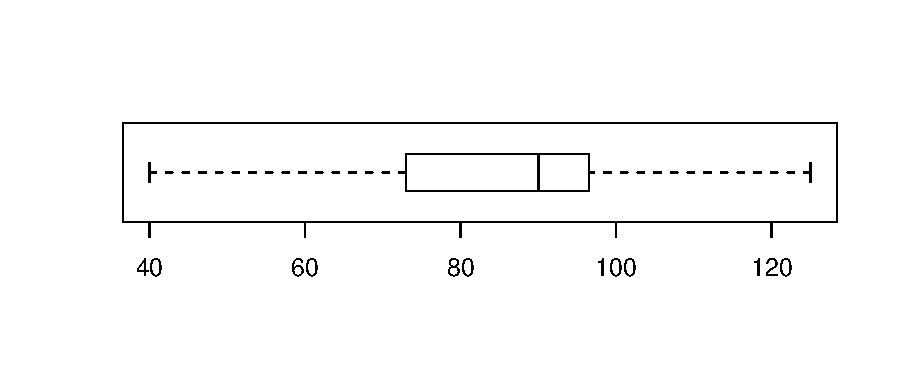
\includegraphics{Devore6-xmp0118}
\end{center}


\section{Example 1.19}
\label{sec:xmp01.19}
\begin{center}
\begin{Schunk}
\begin{Sinput}
> with(xmp01.19, boxplot(C1, horizontal = TRUE))
\end{Sinput}
\end{Schunk}
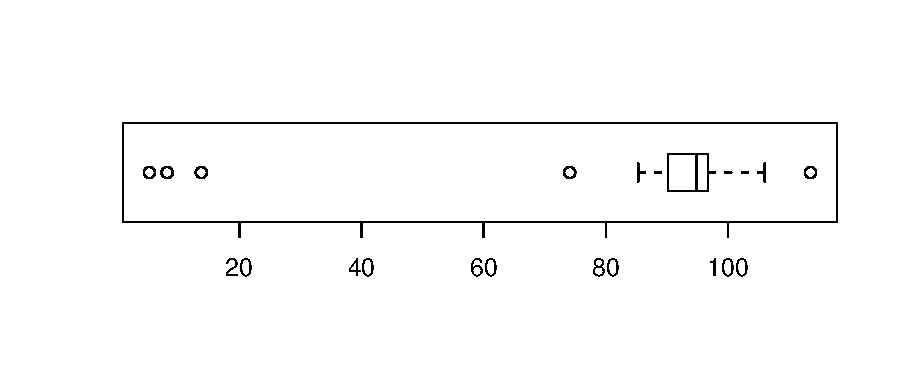
\includegraphics{Devore6-xmp0119}
\end{center}


\section{Comparative boxplots}
\label{sec:xmp0120}

The data for Example~1.20 (p.~43) are not available so we use the data
on scores for creamy and crunchy peanut butters (exercise~1.15, p.~24)
to illustrate comparative boxplots.  This data set has two columns and
37 rows.  The score is the first column and the indicator of
``Creamy'' or ``Crunchy'' is the second column.  We say that these
data are in the stacked format (see Appendix~\ref{app:stacked} for
details).  In the call to \texttt{boxplot} we use the formula
~ to indicate that \texttt{Score} is the response
and \texttt{Type} defines the groups for the comparative boxplot.
\begin{center}
\begin{Schunk}
\begin{Sinput}
> with(ex01.15, boxplot(Score ~ Type, horizontal = TRUE, las = 1))
\end{Sinput}
\end{Schunk}
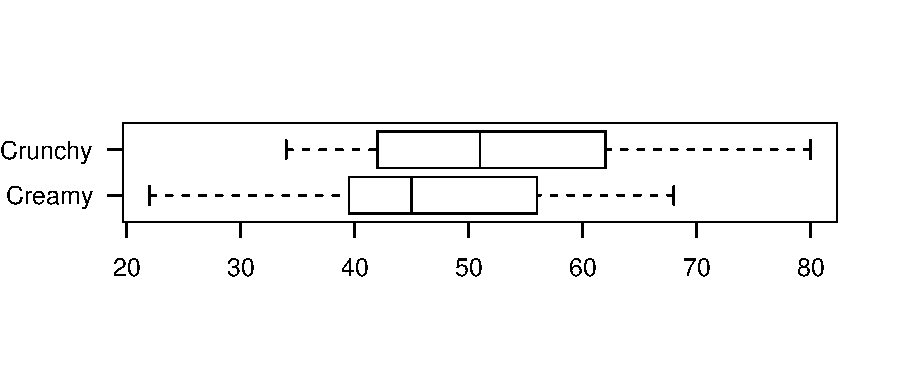
\includegraphics{Devore6-xmp0120}
\end{center}

\section{Enhancing graphical displays}
\label{sec:ch1enhance}

In this chapter we have used several functions, such as \texttt{hist},
\texttt{barplot}, \texttt{plot}, and \texttt{boxplot} that produce
graphical displays of data.  These functions all can take optional
arguments that provide more effective displays.  For example, in
\S~\ref{sec:xmp0120}, we used the optional argument \texttt{las=1} to
\texttt{boxplot} to change the label style on the vertical axis so the
labels are horizontal rather than vertical.

The \texttt{las=1} argument can be used with other graphics functions.
Compare
\begin{center}
\begin{Schunk}
\begin{Sinput}
> with(xmp01.10, hist(consump, las = 1))
\end{Sinput}
\end{Schunk}
\includegraphics{Devore6-030}
\end{center}
with the display in \S~\ref{sec:xmp01.10}

We have also seen how the \texttt{breaks} argument can be used with
\texttt{hist} and how the \texttt{scale} argument can be used with
\texttt{stem}.  To reproduce a display like Figure~1.5 (p.~5) we would
use
\begin{Schunk}
\begin{Sinput}
> with(xmp01.01, stem(temp, scale = 2))
\end{Sinput}
\begin{Soutput}
  The decimal point is 1 digit(s) to the right of the |

  3 | 1
  3 | 
  4 | 0
  4 | 59
  5 | 23
  5 | 788
  6 | 0113
  6 | 6777789
  7 | 000023
  7 | 556689
  8 | 0134
\end{Soutput}
\end{Schunk}
and
\begin{Schunk}
\begin{Sinput}
> with(xmp01.01, hist(temp, breaks = c(25, 35, 45, 55, 65, 
+     75, 85)))
\end{Sinput}
\end{Schunk}
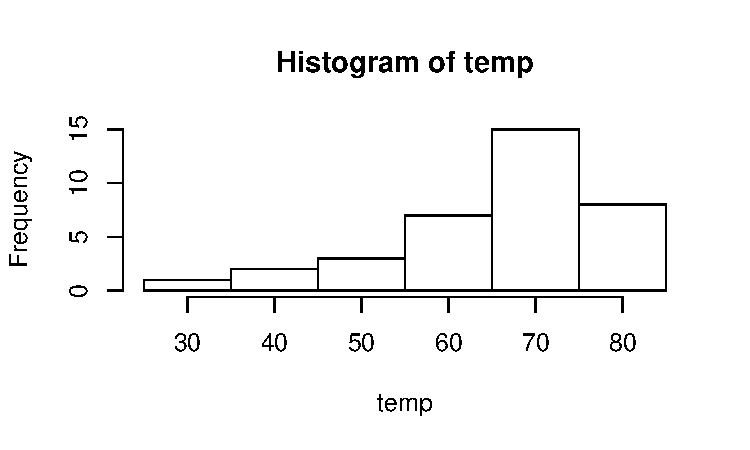
\includegraphics{Devore6-032}

\chapter{Probability}
\label{ch:Probability}

Table~\ref{tab:ch2} lists a function used in chapter 2.
\begin{table}[htbp]
  \centering
  \begin{tabular}{l l}
    \multicolumn{1}{c}{\textbf{Function}} &
    \multicolumn{1}{c}{\textbf{Description}} \\
    \hline
    choose(n,k)   & calculate $\binom{n}{k}$\\
    \hline
  \end{tabular}
  \caption{R functions used in chapter 2}
  \label{tab:ch2}
\end{table}


\section{Example 2.23}
\label{sec:xmp0223}

In this chapter on probability there is little use for R functions
except for the \texttt{choose} function that evaluates the number of
combinations of $k$ objects selected from $n$, written $\binom{n}{k}$
and described in section~2.3 (pp.~71--73).  To calculate the first
probability in example 2.23 (p.~73)
\begin{Schunk}
\begin{Sinput}
> choose(15, 3) * choose(10, 3)/choose(25, 6)
\end{Sinput}
\begin{Soutput}
[1] 0.3083004
\end{Soutput}
\end{Schunk}


\chapter[Discrete Random Variables]{Discrete Random Variables and
  Probability Distributions}
\label{cha:Discrete}

To quote the document ``Introduction to R''
\begin{quote}
     One convenient use of R is to provide a comprehensive set of
statistical tables.  Functions are provided to evaluate the cumulative
distribution function P(X <= x), the probability density function and
the quantile function (given q, the smallest x such that P(X <= x) > q),
and to simulate from the distribution.
\begin{center}
  \begin{tabular}{l l l}
    \multicolumn{1}{c}{Distribution}&
    \multicolumn{1}{c}{R name}&
    \multicolumn{1}{c}{additional arguments}\\\hline
    binomial& `binom'& `size, prob'\\
    geometric& `geom' & `prob'\\
    hypergeometric&`hyper'&`m, n, k'\\
    negative binomial&`nbinom'&`size, prob'\\
    Poisson&`pois'&`lambda'\\
    \hline
  \end{tabular}
\end{center}

Prefix the name given here by `d' for the density, `p' for the CDF, `q'
for the quantile function and `r' for simulation (\textbf{r}andom deviates).
The first argument is `x' for `dXXX', `q' for `pXXX', `p' for `qXXX'
and `n' for `rXXX' (except for `rhyper' and `rwilcox', for which it is
`nn').
\end{quote}

These functions are more versatile and more accurate than using
probability tables.

\section{Example 3.30}
\label{sec:xmp0330}
For $X$ having a binomial distribution with $n=6$ and $p=0.5$ we are
to calculate $P(X=3)$, $P(3\le X)$, and $P(X\le 1)$.
\begin{Schunk}
\begin{Sinput}
> dbinom(3, size = 6, prob = 0.5)
\end{Sinput}
\begin{Soutput}
[1] 0.3125
\end{Soutput}
\begin{Sinput}
> dbinom(3:6, size = 6, prob = 0.5)
\end{Sinput}
\begin{Soutput}
[1] 0.312500 0.234375 0.093750 0.015625
\end{Soutput}
\begin{Sinput}
> sum(dbinom(3:6, size = 6, prob = 0.5))
\end{Sinput}
\begin{Soutput}
[1] 0.65625
\end{Soutput}
\begin{Sinput}
> 1 - pbinom(2, size = 6, prob = 0.5)
\end{Sinput}
\begin{Soutput}
[1] 0.65625
\end{Soutput}
\begin{Sinput}
> pbinom(2, size = 6, prob = 0.5, lower = FALSE)
\end{Sinput}
\begin{Soutput}
[1] 0.65625
\end{Soutput}
\begin{Sinput}
> pbinom(1, 6, 0.5)
\end{Sinput}
\begin{Soutput}
[1] 0.109375
\end{Soutput}
\end{Schunk}
The first call evaluates $b(3; 6, .5)$. The second call evaluates the
probability function at $3,\dots,6$ using the \texttt{":"} operator
that generates the sequence from 3 to 6.  If we sum this vector of
probabilities we get $P(3\le X)$.  An alternative is to use $P(3\le
X)=1-P(X\le2)$ and evaluate $P(X\le 2)$ with \texttt{pbinom}.  Another
alternative is to use cumulative probability in the upper tail,
obtained with the optional argument \texttt{lower=FALSE} to
\texttt{pbinom}.  Finally \texttt{pbinom} is used to calculate $P(X\le
1)$.
\section{Example 3.31}
\begin{Schunk}
\begin{Sinput}
> pbinom(8, 15, 0.2)
\end{Sinput}
\begin{Soutput}
[1] 0.999215
\end{Soutput}
\begin{Sinput}
> dbinom(8, 15, 0.2)
\end{Sinput}
\begin{Soutput}
[1] 0.003454764
\end{Soutput}
\begin{Sinput}
> 1 - pbinom(7, 15, 0.2)
\end{Sinput}
\begin{Soutput}
[1] 0.00423975
\end{Soutput}
\begin{Sinput}
> sum(dbinom(4:7, 15, 0.2))
\end{Sinput}
\begin{Soutput}
[1] 0.3475981
\end{Soutput}
\end{Schunk}
\section{Example 3.34}
R uses a different, but equivalent, set of parameters for the
hypergeometric distribution than does
the text.  In the text the parameters of the hypergeometric are $N$,
the population size, $n$, the sample size, and $M$, the number of
``successes'' in the population.  In R the sample size is called $k$,
the parameter $m$ corresponds to $M$ in the text, and $n$ is $N-M$.

Thus what is written in the text as $h(2;5,12,20)$ becomes
\begin{Schunk}
\begin{Sinput}
> dhyper(2, 12, 8, 5)
\end{Sinput}
\begin{Soutput}
[1] 0.2383901
\end{Soutput}
\end{Schunk}

\section{Example 3.35}
\label{sec:xmp0335}

\begin{Schunk}
\begin{Sinput}
> dhyper(2, 5, 20, 10)
\end{Sinput}
\begin{Soutput}
[1] 0.3853755
\end{Soutput}
\begin{Sinput}
> phyper(2, 5, 20, 10)
\end{Sinput}
\begin{Soutput}
[1] 0.6988142
\end{Soutput}
\end{Schunk}


\section{Example 3.37}
\label{sec:xmp0337}

The negative binomial density function, \texttt{dnbinom}, shown in the
text as $nb(10; 5, 2)$, has essentially the same calling sequence in
R.  The cumulative probability function is \texttt{pnbinom}.
\begin{Schunk}
\begin{Sinput}
> dnbinom(10, 5, 0.2)
\end{Sinput}
\begin{Soutput}
[1] 0.0343941
\end{Soutput}
\begin{Sinput}
> pnbinom(10, 5, 0.2)
\end{Sinput}
\begin{Soutput}
[1] 0.1642337
\end{Soutput}
\end{Schunk}


\section{Example 3.38}
\label{sec:xmp0338}

\begin{Schunk}
\begin{Sinput}
> dpois(5, lambda = 4.5)
\end{Sinput}
\begin{Soutput}
[1] 0.1708269
\end{Soutput}
\begin{Sinput}
> ppois(5, 4.5)
\end{Sinput}
\begin{Soutput}
[1] 0.7029304
\end{Soutput}
\end{Schunk}

\section{Example 3.39}
\label{sec:xmp0339}

The Poisson distribution can be used to approximate binomial
probabilities with large $n$ and small $p$.  However, there is no need
to do so because the exact binomial probabilities can be evaluated.
\begin{Schunk}
\begin{Sinput}
> dbinom(1, 400, 0.005)
\end{Sinput}
\begin{Soutput}
[1] 0.2706694
\end{Soutput}
\begin{Sinput}
> dpois(1, 2)
\end{Sinput}
\begin{Soutput}
[1] 0.2706706
\end{Soutput}
\begin{Sinput}
> pbinom(3, 400, 0.005)
\end{Sinput}
\begin{Soutput}
[1] 0.8575767
\end{Soutput}
\begin{Sinput}
> ppois(3, 2)
\end{Sinput}
\begin{Soutput}
[1] 0.8571235
\end{Soutput}
\end{Schunk}

\chapter[Continuous Random Variables]{Continuous Random Variables and
  Probability Distributions}
\label{cha:Continuous}

The set of continous distributions available in R is
\begin{center}
  \begin{tabular}{l l l}
    \multicolumn{1}{c}{Distribution}&
    \multicolumn{1}{c}{R name}&
    \multicolumn{1}{c}{additional arguments}\\\hline
    beta          & `beta'   &  `shape1, shape2, ncp' \\
    Cauchy        & `cauchy' & `location, scale'  \\
    $\chi^2$       & `chisq'  & `df, ncp' \\
    exponential   & `exp'    & `rate' \\
    F             & `f'      & `df1, df1, ncp' \\
    gamma         & `gamma'  & `shape, scale' \\
    log-normal    & `lnorm'  & `meanlog, sdlog' \\
    logistic      & `logis'  & `location, scale' \\
    normal        & `norm'   & `mean, sd' \\
    Student's t   & `t'      & `df, ncp' \\
    uniform       & `unif'   & `min, max' \\
    Weibull       & `weibull'& `shape, scale'\\
    Wilcoxon      & `wilcox' & `m, n'\\
    \hline
  \end{tabular}
\end{center}

As with the discrete distributions, prefix the name given here by `d'
for the density, `p' for the CDF, `q' for the quantile function and
`r' for simulation (\textbf{r}andom deviates).  The first argument is
`x' for `dXXX', `q' for `pXXX', `p' for `qXXX' and `n' for `rXXX'

Not all the distributions shown above are discussed in the text.


\section{Example 4.12}
\label{sec:xmp0412}

Function \texttt{pnorm} provides the standard normal cumulative
distribution function by default.  The optional arguments
\texttt{mean} and \texttt{sd} can be set to values other than 0 and 1
to provide probabilities from any normal distribution.

$P(Z\le 1.25)$ and $P(Z\le-1.25)$ are evaluated as
\begin{Schunk}
\begin{Sinput}
> pnorm(1.25)
\end{Sinput}
\begin{Soutput}
[1] 0.8943502
\end{Soutput}
\begin{Sinput}
> pnorm(-1.25)
\end{Sinput}
\begin{Soutput}
[1] 0.1056498
\end{Soutput}
\end{Schunk}
$P(Z>1.25)$ can be evaluated in two ways
\begin{Schunk}
\begin{Sinput}
> 1 - pnorm(1.25)
\end{Sinput}
\begin{Soutput}
[1] 0.1056498
\end{Soutput}
\begin{Sinput}
> pnorm(1.25, lower = FALSE)
\end{Sinput}
\begin{Soutput}
[1] 0.1056498
\end{Soutput}
\end{Schunk}
To evaluate probabilities of intervals, such as $P(-0.38\le
Z\le1.25)$, apply \texttt{pnorm} to the endpoints as a vector (created
with the \texttt{"c"} function) which returns a vector of
probabilities.  The \texttt{"diff"} function forms successive
differences from which we obtain the probability in the interval.
\begin{Schunk}
\begin{Sinput}
> pnorm(c(-0.38, 1.25))
\end{Sinput}
\begin{Soutput}
[1] 0.3519727 0.8943502
\end{Soutput}
\begin{Sinput}
> diff(pnorm(c(-0.38, 1.25)))
\end{Sinput}
\begin{Soutput}
[1] 0.5423775
\end{Soutput}
\end{Schunk}


\section{Example 4.13}
\label{sec:xmp0413}

The inverse of the standard normal CDF, called the quantile function,
is obtained with \texttt{qnorm}.  Notice that the first argument to
\texttt{qnorm} is a probability, not a percentage.
\begin{Schunk}
\begin{Sinput}
> qnorm(0.99)
\end{Sinput}
\begin{Soutput}
[1] 2.326348
\end{Soutput}
\end{Schunk}

\section{Example 4.14}
\label{sec:xmp0414}

To obtain $z_\alpha$, use the optional argument \texttt{lower=FALSE}
to \texttt{qnorm}.
\begin{Schunk}
\begin{Sinput}
> qnorm(0.05, lower = FALSE)
\end{Sinput}
\begin{Soutput}
[1] 1.644854
\end{Soutput}
\end{Schunk}

\section{Example 4.15}
\label{sec:xmp0415}

Nonstandard normal distribution probabilities or quantiles are
obtained with the optional arguments \texttt{mean} and \texttt{sd} to
\texttt{pnorm} and \texttt{qnorm}.  In this example $\mu=1.25$ and
$\sigma=0.46$ and we wish to evaluate $P(1.00\le X\le 1.75)$
\begin{Schunk}
\begin{Sinput}
> diff(pnorm(c(1, 1.75), mean = 1.25, sd = 0.46))
\end{Sinput}
\begin{Soutput}
[1] 0.5680717
\end{Soutput}
\end{Schunk}


\section{Example 4.17}
\label{sec:xmp0417}

For $\mu=64$ and $\sigma=0.78$, the 99.5th percentile is
\begin{Schunk}
\begin{Sinput}
> qnorm(0.995, mean = 64, sd = 0.78)
\end{Sinput}
\begin{Soutput}
[1] 66.00915
\end{Soutput}
\end{Schunk}


\section{Example 4.19}
\label{sec:xmp0419}

The normal approximation to binomial probabilities can be calculated
but, like the Poisson approximation, it is not necessary as the exact
binomial probabilities can also be calculated.
\begin{Schunk}
\begin{Sinput}
> pnorm(10.5, mean = 12.5, sd = sqrt(12.5 * 0.75))
\end{Sinput}
\begin{Soutput}
[1] 0.2568146
\end{Soutput}
\begin{Sinput}
> pbinom(10, size = 50, prob = 0.25)
\end{Sinput}
\begin{Soutput}
[1] 0.2622023
\end{Soutput}
\begin{Sinput}
> diff(pnorm(c(4.5, 15.5), mean = 12.5, sd = sqrt(12.5 * 0.75)))
\end{Sinput}
\begin{Soutput}
[1] 0.8319162
\end{Soutput}
\begin{Sinput}
> diff(pbinom(c(4, 15), size = 50, prob = 0.25))
\end{Sinput}
\begin{Soutput}
[1] 0.8348084
\end{Soutput}
\end{Schunk}


\section{Example 4.20}
\label{sec:xmp0420}

The parameters $\alpha$ and $\beta$ of the gamma distribution are named
\texttt{shape} and \texttt{scale} respectively in R.
In this example $\alpha=2$ and $\beta$ has the default value of 1.
\begin{Schunk}
\begin{Sinput}
> pgamma(c(3, 5), shape = 2)
\end{Sinput}
\begin{Soutput}
[1] 0.8008517 0.9595723
\end{Soutput}
\begin{Sinput}
> diff(pgamma(c(3, 5), shape = 2))
\end{Sinput}
\begin{Soutput}
[1] 0.1587206
\end{Soutput}
\begin{Sinput}
> pgamma(4, shape = 2, lower = FALSE)
\end{Sinput}
\begin{Soutput}
[1] 0.0915782
\end{Soutput}
\end{Schunk}


\section{Example 4.21}
\label{sec:xmp0421}

\begin{Schunk}
\begin{Sinput}
> diff(pgamma(c(60, 120), shape = 8, scale = 15))
\end{Sinput}
\begin{Soutput}
[1] 0.4959056
\end{Soutput}
\begin{Sinput}
> pgamma(30, shape = 8, scale = 15, lower = FALSE)
\end{Sinput}
\begin{Soutput}
[1] 0.9989033
\end{Soutput}
\end{Schunk}


\section{Examples 4.22 and 4.23}
\label{sec:xmp0422}

In R the parameter $\lambda$ of the exponential distribution is called
\texttt{rate}
\begin{Schunk}
\begin{Sinput}
> pexp(10, rate = 0.2)
\end{Sinput}
\begin{Soutput}
[1] 0.8646647
\end{Soutput}
\begin{Sinput}
> diff(pexp(c(5, 10), rate = 0.2))
\end{Sinput}
\begin{Soutput}
[1] 0.2325442
\end{Soutput}
\begin{Sinput}
> pexp(2, rate = 0.5, lower = FALSE)
\end{Sinput}
\begin{Soutput}
[1] 0.3678794
\end{Soutput}
\end{Schunk}

\section{Example 4.24}
\label{sec:xmp0424}

The parameters $\alpha$ and $\beta$ of the Weibull distribution are
called \texttt{shape} and \texttt{scale}.
\begin{Schunk}
\begin{Sinput}
> pweibull(10, shape = 2, scale = 10)
\end{Sinput}
\begin{Soutput}
[1] 0.6321206
\end{Soutput}
\begin{Sinput}
> qweibull(0.95, shape = 2, scale = 10)
\end{Sinput}
\begin{Soutput}
[1] 17.30818
\end{Soutput}
\end{Schunk}


\section{Example 4.26}
\label{sec:xmp0426}

The lognormal distribution takes two parameters named \texttt{meanlog}
and \texttt{sdlog}.
\begin{Schunk}
\begin{Sinput}
> diff(plnorm(c(1, 2), meanlog = 0.375, sdlog = 0.25))
\end{Sinput}
\begin{Soutput}
[1] 0.8316108
\end{Soutput}
\begin{Sinput}
> qlnorm(0.99, meanlog = 0.375, sdlog = 0.25)
\end{Sinput}
\begin{Soutput}
[1] 2.602798
\end{Soutput}
\end{Schunk}


\section{Example 4.27}
\label{sec:xmp0427}

R provides probabilities and quantiles of the standard beta
distribution with $A=0$ and $B=1$. The parameters $\alpha$ and $\beta$
are called \texttt{shape1} and \texttt{shape2} respectively.  To use
other values of $A$ and $B$ the scaling must be done manually.  In
this example $A=2$, $B=5$, $\alpha=2$ and $\beta=3$.  To transform to
a standard beta distribution we replace $x$ by $(x-2)/(5-2)$
\begin{Schunk}
\begin{Sinput}
> pbeta((3 - 2)/(5 - 2), shape1 = 2, shape2 = 3)
\end{Sinput}
\begin{Soutput}
[1] 0.4074074
\end{Soutput}
\end{Schunk}


\section{Examples 4.28 and 4.29}
\label{sec:xmp0428}

The normal probability plot is produced with \texttt{qqnorm}.  A
reference line can be added with \texttt{qqline}.
\begin{center}
\setkeys{Gin}{width=0.7\textwidth}
\begin{Schunk}
\begin{Sinput}
> with(xmp04.28, qqnorm(meas.err))
> with(xmp04.28, qqline(meas.err))
\end{Sinput}
\end{Schunk}
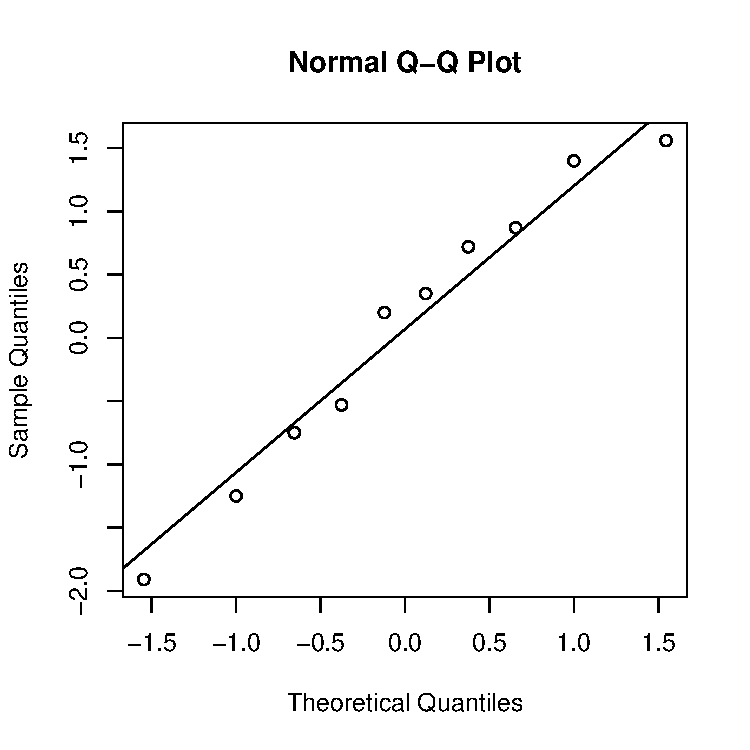
\includegraphics{Devore6-xmp0428}
\end{center}

\begin{center}
\setkeys{Gin}{width=0.7\textwidth}
\begin{Schunk}
\begin{Sinput}
> with(xmp04.29, qqnorm(Voltage))
> with(xmp04.29, qqline(Voltage))
\end{Sinput}
\end{Schunk}
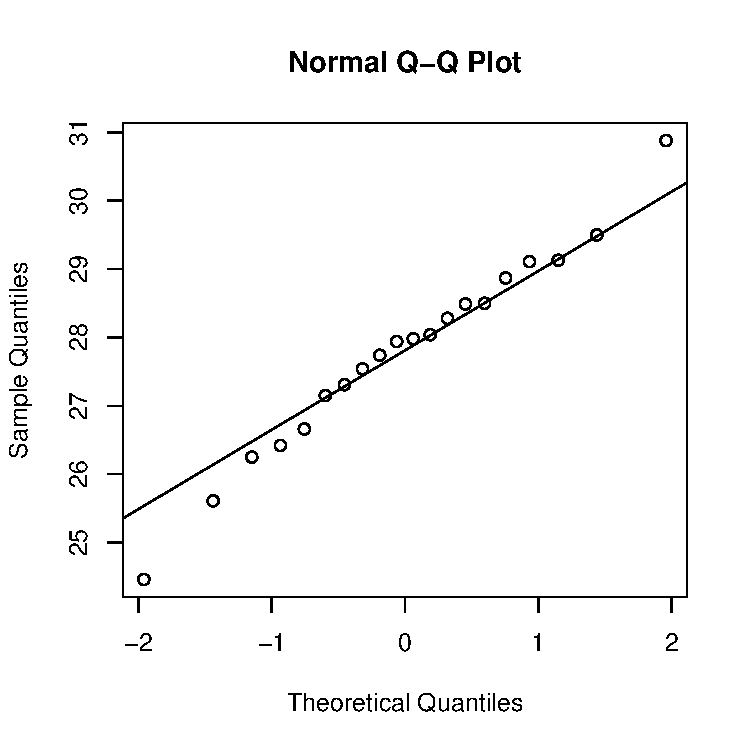
\includegraphics{Devore6-xmp0429}
\end{center}


\section{Example 4.30}
\label{sec:xmp0430}

The Weibull probability plot is not available directly in R.  However,
the plot can be created using the formula $\ln[-\ln(1-p)]$ for the
5th, 15th$,\dots,$ and 95th percentiles as given in text.  The
sequence $0.05,0.15,\dots,0.95$ is generated with
\texttt{seq(0.05, 0.95, 0.1)}.
\begin{Schunk}
\begin{Sinput}
> with(xmp04.30, plot(log(-log(1 - seq(0.05, 0.95, 0.1))), 
+     log(lifetime)))
\end{Sinput}
\end{Schunk}
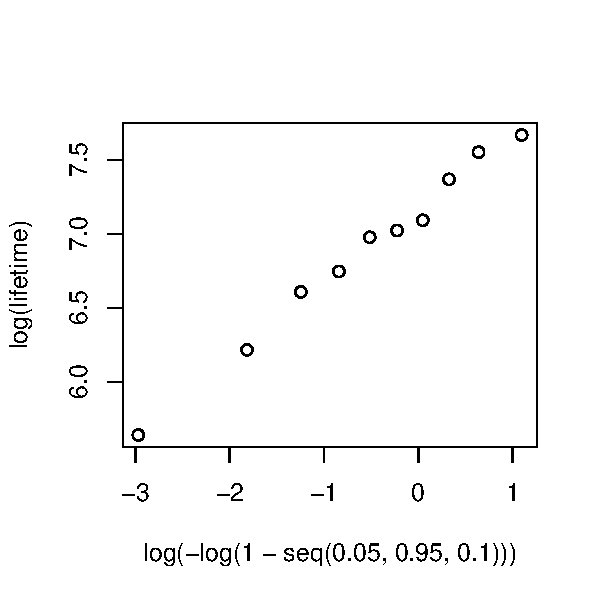
\includegraphics{Devore6-xmp0430}


\chapter[Joint Probability Distributions]{Joint Probability
  Distributions and Random Samples}
\label{cha:Joint}

The main use of R in this chapter is for simulation experiments as
described in section~5.3.

\section{Example 5.19}
\label{sec:xmp0519}

In this example six samples of size ten are drawn from a Weibull
distribution with $\alpha=2$ and $\beta=5$.  To reproduce the plot of
the density shown in Figure 5.6 we can use
\begin{Schunk}
\begin{Sinput}
> curve(dweibull(x, shape = 2, scale = 5), 0, 15, las = 1)
\end{Sinput}
\end{Schunk}
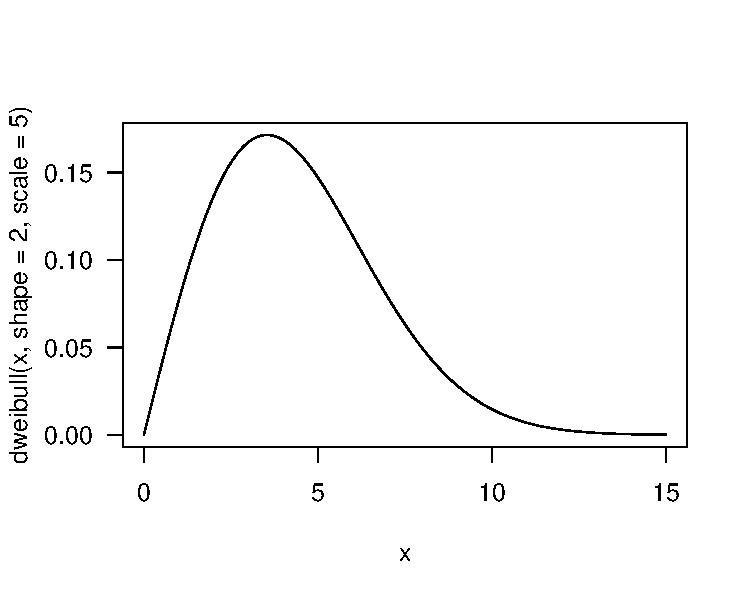
\includegraphics{Devore6-xmp0519a}
To get a single sample of size 10 from this Weibull distribution we use
\begin{Schunk}
\begin{Sinput}
> rweibull(10, shape = 2, scale = 5)
\end{Sinput}
\begin{Soutput}
 [1] 3.35465 1.99426 0.90884 4.78812 8.35764 4.94287 6.66060 6.38006
 [9] 1.83546 9.33432
\end{Soutput}
\end{Schunk}
We could store such a sample as, say, \texttt{samp}, then evaluate its
sample mean, sample median, and sample standard deviation.
\begin{Schunk}
\begin{Sinput}
> samp = rweibull(10, shape = 2, scale = 5)
> print(samp)
\end{Sinput}
\begin{Soutput}
 [1] 2.1045 7.1842 3.0784 4.3427 3.1538 4.2008 8.5321 2.7531 6.4027 4.8325
\end{Soutput}
\begin{Sinput}
> mean(samp)
\end{Sinput}
\begin{Soutput}
[1] 4.6585
\end{Soutput}
\begin{Sinput}
> median(samp)
\end{Sinput}
\begin{Soutput}
[1] 4.2718
\end{Soutput}
\begin{Sinput}
> sd(samp)
\end{Sinput}
\begin{Soutput}
[1] 2.0997
\end{Soutput}
\end{Schunk}
Notice that every time \texttt{rweibull} is called a new sample is generated.

This process of generating a sample and evaluating selected statistics
on the sample could be repeated manually to get a total of 6 samples.
For large simulation experiments this would quickly become tedious so
we put these calculations in a loop.
\begin{Schunk}
\begin{Sinput}
> means = medians = sds = numeric(6)
> for (i in 1:6) {
+     samp = rweibull(10, shape = 2, scale = 5)
+     print(samp)
+     means[i] = mean(samp)
+     medians[i] = median(samp)
+     sds[i] = sd(samp)
+ }
\end{Sinput}
\begin{Soutput}
 [1] 2.4070 4.9239 1.9632 6.8140 6.8132 5.0391 4.9345 5.2769 2.7553 4.8692
 [1] 4.55776 4.18261 4.93903 0.98124 5.16399 4.39556 4.31051 1.68283
 [9] 3.75651 3.88349
 [1]  6.4511  4.7788  2.6227  1.0426 10.7185  1.4989  1.8526  9.8054
 [9]  2.6549  8.1241
 [1] 3.2552 4.9369 5.7727 6.4057 5.4542 2.6201 3.0783 8.6905 1.8143 4.2472
 [1] 12.6809  4.0601  3.9255  6.5601  3.6758  2.7582  5.7285  1.8042
 [9]  0.2857  3.4341
 [1] 6.2628 8.1290 7.3250 5.5068 3.9804 6.1329 6.3925 6.6671 7.6181 7.7674
\end{Soutput}
\begin{Sinput}
> means
\end{Sinput}
\begin{Soutput}
[1] 4.5796 3.7854 4.9550 4.6275 4.4913 6.5782
\end{Soutput}
\begin{Sinput}
> medians
\end{Sinput}
\begin{Soutput}
[1] 4.9292 4.2466 3.7169 4.5921 3.8007 6.5298
\end{Soutput}
\begin{Sinput}
> sds
\end{Sinput}
\begin{Soutput}
[1] 1.6964 1.3715 3.6003 2.0584 3.3843 1.2336
\end{Soutput}
\end{Schunk}
In the first line we assign the names \texttt{means},
\texttt{medians}, and \texttt{sds} to numeric vectors of length 6.
Within the loop we assign individual elements in these vectors.


\section{Example 5.22}
\label{sec:xmp0522}

In this example 500 samples of size $n=5$ are generated from a normal
distribution with $\mu=8.25$ and $\sigma=0.75$ and the mean of each
sample is calculated.  We could do this in a loop, as shown above.
However, it is more compact to generate a matrix with 5 rows and 500
columns then generate a histogram of the means of the columns of this
matrix.  Function \texttt{colMeans} calculates the means of the
columns.  Function \texttt{matrix} creates a matrix from a numeric
vector.  The user can specify the number of rows and the number of
columns.  If one of these is omitted, it is calculated from the length
of the vector and the other dimension.  We set the graphics parameter
\texttt{"mfrow"} (multiple figures by row) to create a 2 by 2 array of
plots.
\begin{Schunk}
\begin{Sinput}
> par(mfrow = c(2, 2))
> samp5 = matrix(rnorm(500 * 5, mean = 8.25, sd = 0.75), ncol = 500)
> hist(colMeans(samp5), main = "Samples of size 5")
> samp10 = matrix(rnorm(500 * 10, mean = 8.25, sd = 0.75), 
+     ncol = 500)
> hist(colMeans(samp10), main = "Samples of size 10")
> samp20 = matrix(rnorm(500 * 20, mean = 8.25, sd = 0.75), 
+     ncol = 500)
> hist(colMeans(samp20), main = "Samples of size 20")
> samp30 = matrix(rnorm(500 * 30, mean = 8.25, sd = 0.75), 
+     ncol = 500)
> hist(colMeans(samp30), main = "Samples of size 30")
\end{Sinput}
\end{Schunk}
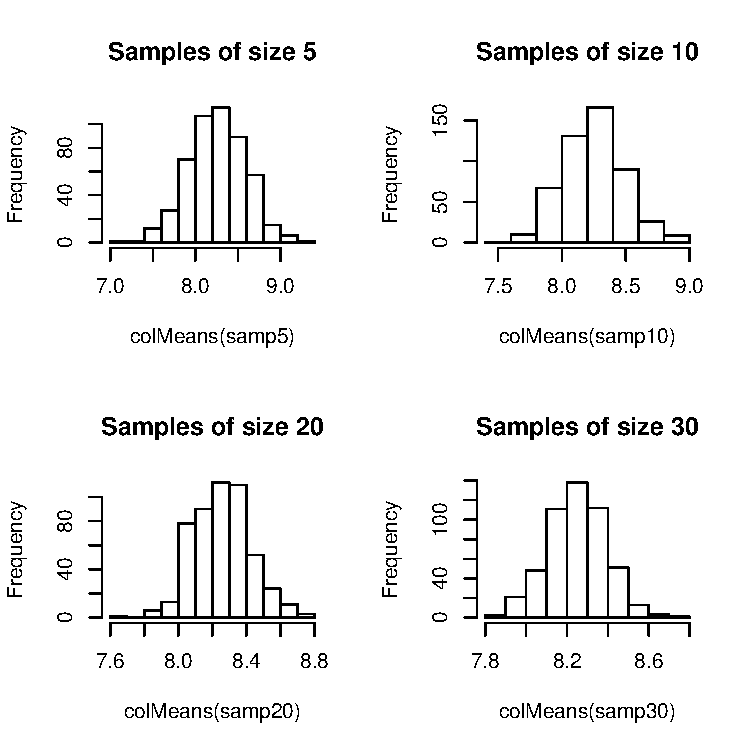
\includegraphics{Devore6-xmp0522a}


\section{Example 5.23}
\label{sec:xmp0523}

This example is similar to Example 5.22.  To reproduce Figure 5.12 use
\begin{Schunk}
\begin{Sinput}
> curve(dlnorm(x, meanlog = 3, sdlog = 0.4), from = 0, to = 75, 
+     las = 1)
\end{Sinput}
\end{Schunk}
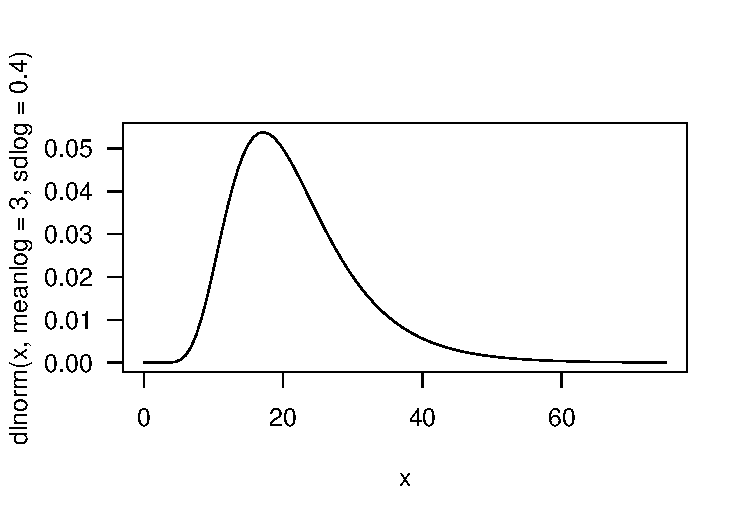
\includegraphics{Devore6-xmp0523a}
The samples and the histograms of the means are generated from
\begin{Schunk}
\begin{Sinput}
> par(mfrow = c(2, 2))
> samp5 = matrix(rlnorm(500 * 5, 2, 0.4), ncol = 500)
> hist(colMeans(samp5), main = "Means of samples of size 5")
> samp10 = matrix(rlnorm(500 * 10, 2, 0.4), ncol = 500)
> hist(colMeans(samp10), main = "Means of samples of size 10")
> samp20 = matrix(rlnorm(500 * 20, 2, 0.4), ncol = 500)
> hist(colMeans(samp20), main = "Means of samples of size 20")
> samp30 = matrix(rlnorm(500 * 30, 2, 0.4), ncol = 500)
> hist(colMeans(samp30), main = "Means of samples of size 30")
\end{Sinput}
\end{Schunk}
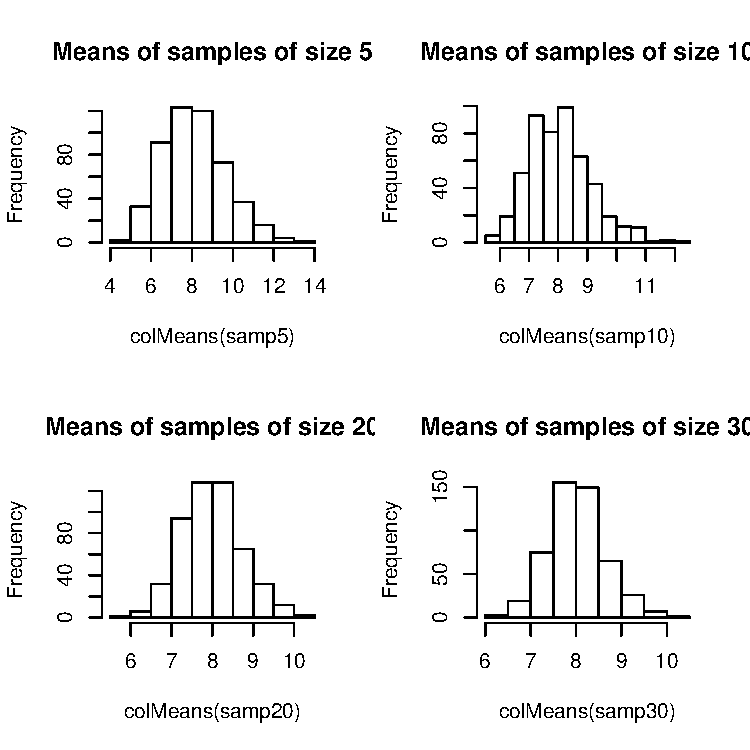
\includegraphics{Devore6-xmp0523b}
Finally the normal probability plot is generated by
\begin{center}
\setkeys{Gin}{width=0.7\textwidth}
\begin{Schunk}
\begin{Sinput}
> qqnorm(colMeans(samp30))
> qqline(colMeans(samp30))
\end{Sinput}
\end{Schunk}
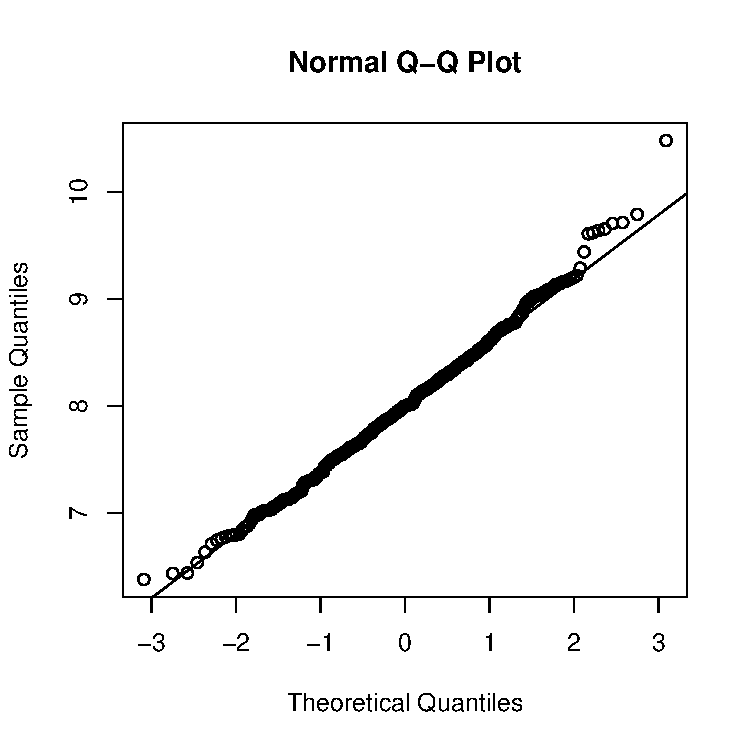
\includegraphics{Devore6-xmp0523c}
\end{center}


\chapter{Point Estimation}
\label{cha:PointEst}


\section{Example 6.2}
\label{sec:xmp0602}
The various estimators of location described in Example 6.2 (p.~255)
can be evaluated as
\begin{Schunk}
\begin{Sinput}
> with(xmp06.02, mean(Voltage))
\end{Sinput}
\begin{Soutput}
[1] 27.793
\end{Soutput}
\begin{Sinput}
> with(xmp06.02, median(Voltage))
\end{Sinput}
\begin{Soutput}
[1] 27.96
\end{Soutput}
\begin{Sinput}
> with(xmp06.02, mean(range(Voltage)))
\end{Sinput}
\begin{Soutput}
[1] 27.67
\end{Soutput}
\begin{Sinput}
> with(xmp06.02, mean(Voltage, trim = 0.1))
\end{Sinput}
\begin{Soutput}
[1] 27.83812
\end{Soutput}
\end{Schunk}

\section{Example 6.3}
\label{sec:xmp0603}

Functions \texttt{var} and \texttt{sd} provide $s^2$ and $s$, the
sample variance and standard deviation, respectively.
\begin{Schunk}
\begin{Sinput}
> with(xmp06.03, var(Strength))
\end{Sinput}
\begin{Soutput}
[1] 0.25125
\end{Soutput}
\begin{Sinput}
> with(xmp06.03, sd(Strength))
\end{Sinput}
\begin{Soutput}
[1] 0.5012484
\end{Soutput}
\end{Schunk}
To evaluate the alternative estimator
$\hat{\sigma}=\frac{\sum\left(X_i-\bar{X}\right)}{n}$ we must evaluate
the formula
\begin{Schunk}
\begin{Sinput}
> with(xmp06.03, sum((Strength - mean(Strength))^2)/length(Strength))
\end{Sinput}
\begin{Soutput}
[1] 0.2198438
\end{Soutput}
\end{Schunk}
Function \texttt{length} applied to a vector returns $n$, the number
of elements in the vector.


\section{Example 6.12}
\label{sec:xmp0612}

The calculation of the method of moments estimates in Example 6.12
(p.~270) can be split into stages
\begin{Schunk}
\begin{Sinput}
> xbar = with(xmp06.12, mean(Survival))
> xsqb = with(xmp06.12, mean(Survival^2))
> xbar
\end{Sinput}
\begin{Soutput}
[1] 113.45
\end{Soutput}
\begin{Sinput}
> xsqb
\end{Sinput}
\begin{Soutput}
[1] 14087.75
\end{Soutput}
\begin{Sinput}
> xbar^2/(xsqb - xbar^2)
\end{Sinput}
\begin{Soutput}
[1] 10.57725
\end{Soutput}
\begin{Sinput}
> (xsqb - xbar^2)/xbar
\end{Sinput}
\begin{Soutput}
[1] 10.72585
\end{Soutput}
\end{Schunk}
These estimates are slightly different from those shown in the text
because the intermediate results $\bar{x}$ and $\sum x_i^2/n$ were
rounded in the text.

Maximum likelihood estimates are discussed later in chapter 6.
We can evaluate the maximum likelihood estimates of $\alpha$ and
$\beta$ for this example using the function \texttt{fitdistr} from the
package \texttt{MASS} that supplements the book ``Modern Applied
Statistics with S (4th ed)'' by Bill Venables and Brian Ripley
(Springer, 2002).  These estimates are determined by numerical
optimization of the logarithm of the likelihood function and we must
supply starting estimates.  We use the method of moments estimates for
this.
\begin{Schunk}
\begin{Sinput}
> library(MASS)
> with(xmp06.12, fitdistr(Survival, dgamma, list(shape = 10.577, 
+     scale = 10.726)))
\end{Sinput}
\begin{Soutput}
     shape       scale  
   8.792026   12.904674 
 ( 2.732520) ( 4.127671)
\end{Soutput}
\end{Schunk}
The MLEs are quite different from the method of moments estimates.
The numbers in parentheses under the estimates are their standard errors.


\chapter[Statistical Intervals]{Statistical Intervals Based on a Single Sample}
\label{cha:Intervals}

Table~\ref{tab:ch7} lists functions used in
chapters~\ref{cha:Intervals} and \ref{cha:Tests}.
\begin{table}[htbp]
  \centering
  \begin{tabular}{l l}
    \multicolumn{1}{c}{\textbf{Function}} &
    \multicolumn{1}{c}{\textbf{Description}} \\\hline
    t.test(x)        & Student's t test and confidence interval\\
    prop.test(x,n)   & Test and confidence interval on proportion\\
    binom.test(x,n)  & Test and confidence interval on proportion\\
    \hline
  \end{tabular}
  \caption{R functions used with chapters~\ref{cha:Intervals} and
    \ref{cha:Tests}}
  \label{tab:ch7}
\end{table}

\section{Example 7.2}
\label{sec:xmp07.02}

The calculation of the confidence interval for known $\sigma$, shown in
Example 7.2, could be done in R as
\begin{Schunk}
\begin{Sinput}
> 80 + c(-1, 1) * 1.96 * 2/sqrt(31)
\end{Sinput}
\begin{Soutput}
[1] 79.29595 80.70405
\end{Soutput}
\end{Schunk}
but it is probably just as easy to use a hand calculator for this.


\section{Example 7.6}
\label{sec:xmp07.06}

The calculation of the sample mean, the sample standard deviation, and
the sample size can be combined into a single statement
\begin{Schunk}
\begin{Sinput}
> with(xmp07.06, mean(Voltage) + c(-1, 1) * 1.96 * sd(Voltage)/sqrt(length(Voltage)))
\end{Sinput}
\begin{Soutput}
[1] 53.22857 56.18810
\end{Soutput}
\end{Schunk}
An alternative, and preferred way, of calculating the interval is to
use \texttt{t.test}.  With 48 observations the confidence interval on
$\mu$ from the t distribution is nearly identical to that from the
standard normal distribution.
\begin{Schunk}
\begin{Sinput}
> with(xmp07.06, t.test(Voltage))
\end{Sinput}
\begin{Soutput}
	One Sample t-test

data:  Voltage 
t = 72.4631, df = 47, p-value = < 2.2e-16
alternative hypothesis: true mean is not equal to 0 
95 percent confidence interval:
 53.18950 56.22716 
sample estimates:
mean of x 
 54.70833 
\end{Soutput}
\end{Schunk}

It is always a good idea to check the normal probability plot when
using \texttt{t.test}, even with a large sample.
\begin{center}
\setkeys{Gin}{width=0.7\textwidth}
\begin{Schunk}
\begin{Sinput}
> with(xmp07.06, qqnorm(Voltage))
\end{Sinput}
\end{Schunk}
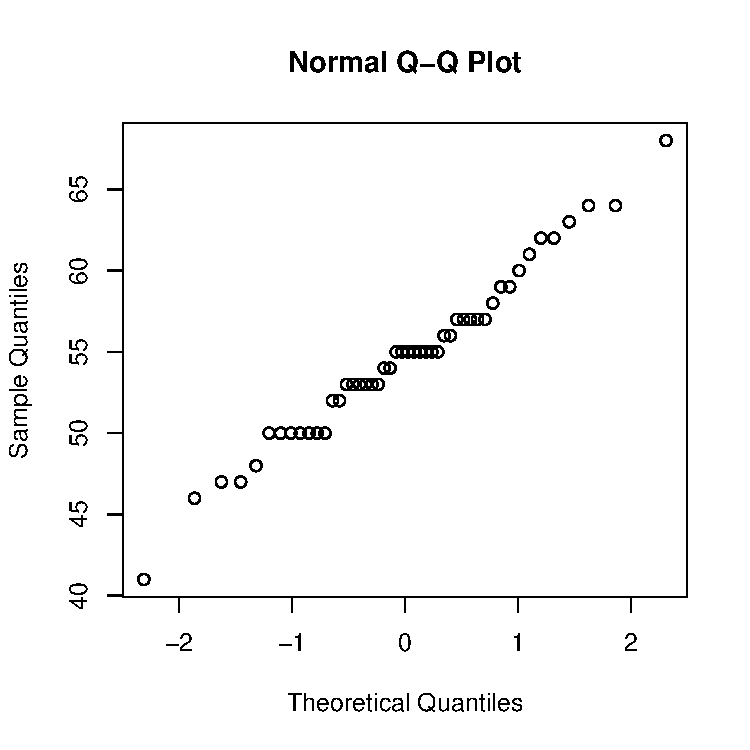
\includegraphics{Devore6-xmp0706c}
\end{center}


\section{Example 7.8}
\label{sec:xmp0708}

R has two functions, \texttt{binom.test} and \texttt{prop.test}, that
can be used to calculate a large-sample confidence interval on the
binomial proportion, $p$.  Neither of them corresponds exactly the the
confidence interval described on p.~295.
\begin{Schunk}
\begin{Sinput}
> prop.test(16, 48)
\end{Sinput}
\begin{Soutput}
	1-sample proportions test with continuity correction

data:  16 out of 48, null probability 0.5 
X-squared = 4.6875, df = 1, p-value = 0.03038
alternative hypothesis: true p is not equal to 0.5 
95 percent confidence interval:
 0.2080794 0.4851357 
sample estimates:
        p 
0.3333333 
\end{Soutput}
\begin{Sinput}
> binom.test(16, 48)
\end{Sinput}
\begin{Soutput}
	Exact binomial test

data:  16 and 48 
number of successes = 16, number of trials = 48, p-value = 0.02930
alternative hypothesis: true probability of success is not equal to 0.5 
95 percent confidence interval:
 0.2039597 0.4841083 
sample estimates:
probability of success 
             0.3333333 
\end{Soutput}
\end{Schunk}

\section{Example 7.11}
\label{sec:xmp0711}
\begin{center}
\setkeys{Gin}{width=0.7\textwidth}
\begin{Schunk}
\begin{Sinput}
> with(xmp07.11, t.test(Elasticity))
\end{Sinput}
\begin{Soutput}
	One Sample t-test

data:  Elasticity 
t = 28.2778, df = 15, p-value = 1.989e-14
alternative hypothesis: true mean is not equal to 0 
95 percent confidence interval:
 13437.11 15627.89 
sample estimates:
mean of x 
  14532.5 
\end{Soutput}
\begin{Sinput}
> with(xmp07.11, qqnorm(Elasticity))
\end{Sinput}
\end{Schunk}
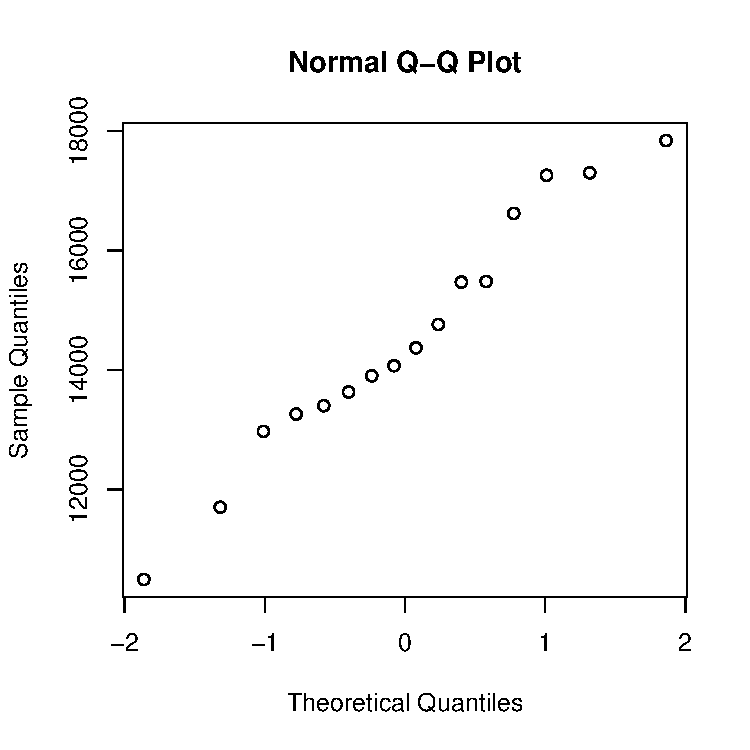
\includegraphics{Devore6-xmp0711a}
\end{center}

\section{Example 7.15}
\label{sec:xmp0715}

Although there is no built-in confidence interval for $\sigma^2$ in R,
the \texttt{qchisq} function can be used to obtain the critical values
$\chi^2_{\alpha/2,n-1}$ and $\chi^2_{1-\alpha/2,n-1}$ used to
calculate the interval.
\begin{center}
\setkeys{Gin}{width=0.7\textwidth}
\begin{Schunk}
\begin{Sinput}
> with(xmp07.15, qqnorm(voltage))
> with(xmp07.15, 16 * var(voltage)/qchisq(c(0.975, 0.025), 
+     df = 16))
\end{Sinput}
\begin{Soutput}
[1]  76171.31 318079.76
\end{Soutput}
\end{Schunk}
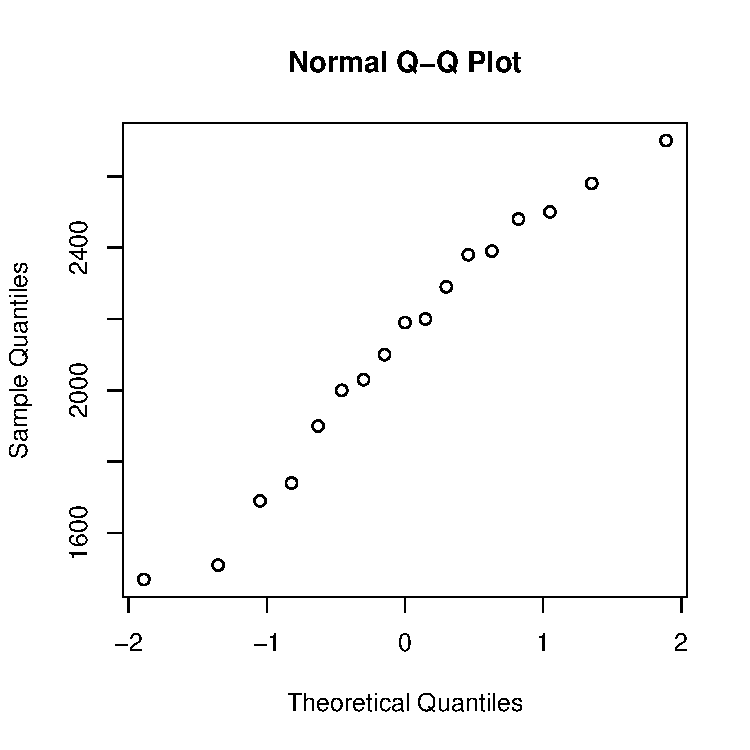
\includegraphics{Devore6-xmp0715}
\end{center}

\chapter[Tests of Hypotheses]{Tests of Hypotheses Based on a Single Sample}
\label{cha:Tests}

The functions described in chapter~\ref{cha:Intervals} are used for
performing tests of hypotheses based on a single sample.  Optional
arguments are used to specify $\mu_0$ or $p_0$ and to indicate the
form of the alternative hypothesis.  All of these tests return a
p-value, described in \S8.4 (pp.~344--350).  From the p-value the
result of the hypothesis test for any level $\alpha$ can be determined.

\section{Example 8.8}
\label{sec:xmp0808}

In R the \texttt{t.test} function can be used with any size of data
set.  For large $n$ the t test is essentially equivalent to the
large-sample z test.
\begin{Schunk}
\begin{Sinput}
> with(xmp08.08, t.test(DCP, mu = 30, alt = "less"))
\end{Sinput}
\begin{Soutput}
	One Sample t-test

data:  DCP 
t = -0.7282, df = 51, p-value = 0.2349
alternative hypothesis: true mean is less than 30 
95 percent confidence interval:
     -Inf 31.61088 
sample estimates:
mean of x 
 28.76154 
\end{Soutput}
\end{Schunk}

As the p-value of 0.2349 exceeds 0.05 we do not reject $H_0:\mu=30$
versus $H_a:\mu < 30$ at level $\alpha=0.05$.

Although not shown in the text book, it is of interest to examine the
normal probability plot for these data
\begin{center}
\setkeys{Gin}{width=0.7\textwidth}
\begin{Schunk}
\begin{Sinput}
> with(xmp08.08, qqnorm(DCP))
\end{Sinput}
\end{Schunk}
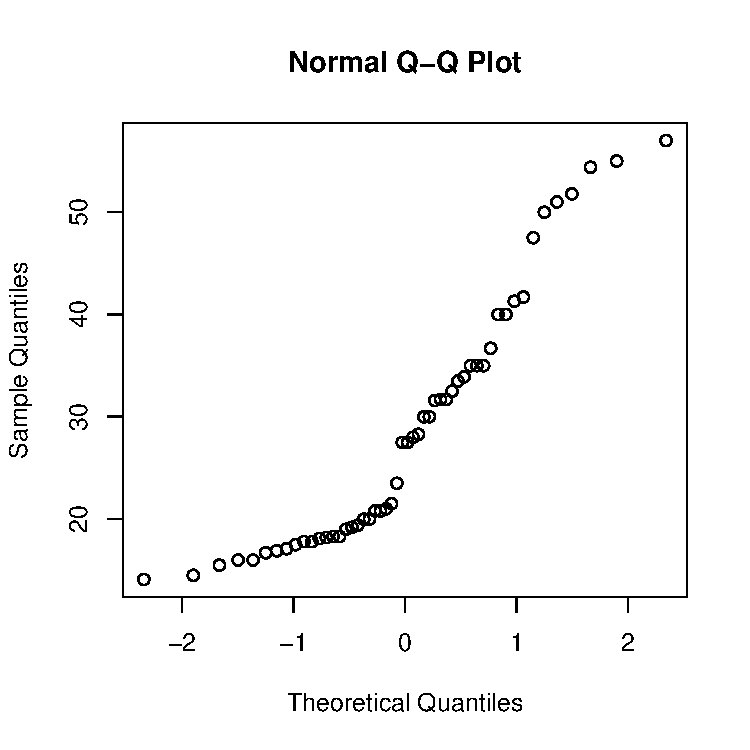
\includegraphics{Devore6-xmp0808b}
\end{center}
This plot shows considerable skewness in the data.  If we transform to
the logarithm of the DCP measurement the skewness is diminished.
\begin{center}
\setkeys{Gin}{width=0.7\textwidth}
\begin{Schunk}
\begin{Sinput}
> with(xmp08.08, qqnorm(log(DCP)))
\end{Sinput}
\end{Schunk}
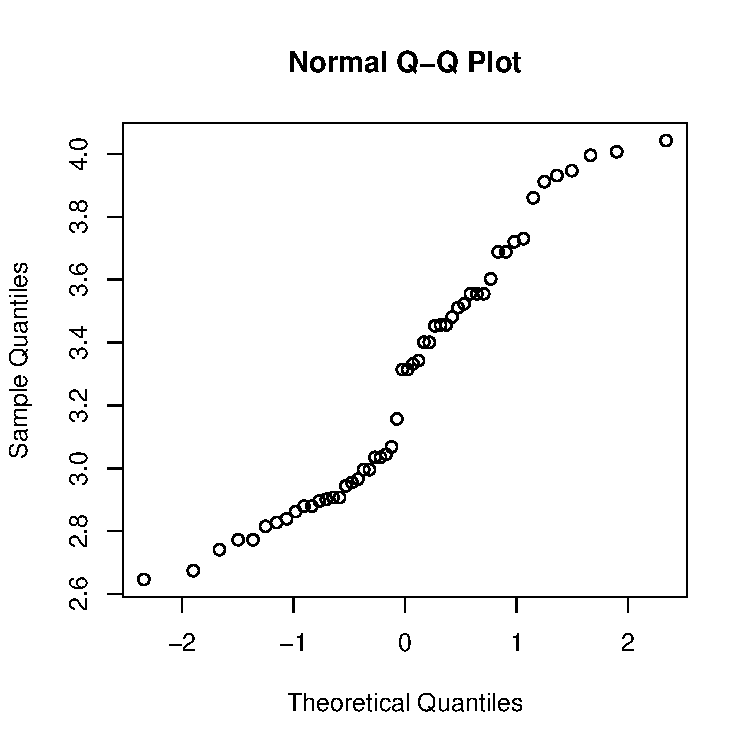
\includegraphics{Devore6-xmp0808c}
\end{center}
and in the logarithm scale, the hypothesis test
$H_0:\mu_\textit{log}=\log(30)$ versus $H_a:\mu_\textit{log}<
\log(30)$ is significant at level $\alpha=0.05$.
\begin{Schunk}
\begin{Sinput}
> with(xmp08.08, t.test(log(DCP), mu = log(30), alt = "less"))
\end{Sinput}
\begin{Soutput}
	One Sample t-test

data:  log(DCP) 
t = -2.223, df = 51, p-value = 0.01534
alternative hypothesis: true mean is less than 3.401197 
95 percent confidence interval:
     -Inf 3.370103 
sample estimates:
mean of x 
 3.274999 
\end{Soutput}
\end{Schunk}

\section{Example 8.9}
\label{sec:xmp0809}

\begin{Schunk}
\begin{Sinput}
> with(xmp08.09, t.test(MAWL, mu = 25, alt = "greater"))
\end{Sinput}
\begin{Soutput}
	One Sample t-test

data:  MAWL 
t = 1.0382, df = 4, p-value = 0.1789
alternative hypothesis: true mean is greater than 25 
95 percent confidence interval:
 22.32433      Inf 
sample estimates:
mean of x 
    27.54 
\end{Soutput}
\end{Schunk}

\section{Example 8.10}
\label{sec:xmp0810}

\begin{Schunk}
\begin{Sinput}
> power.t.test(n = 10, delta = 0.1, sd = 0.1, type = "one.sample", 
+     alt = "one.sided")
\end{Sinput}
\begin{Soutput}
     One-sample t test power calculation 

              n = 10
          delta = 0.1
             sd = 0.1
      sig.level = 0.05
          power = 0.897517
    alternative = one.sided
\end{Soutput}
\begin{Sinput}
> power.t.test(delta = 0.1, sd = 0.1, power = 0.95, type = "one.sample", 
+     alt = "one.sided")
\end{Sinput}
\begin{Soutput}
     One-sample t test power calculation 

              n = 12.32052
          delta = 0.1
             sd = 0.1
      sig.level = 0.05
          power = 0.95
    alternative = one.sided
\end{Soutput}
\end{Schunk}

\section{Example 8.11}
\label{sec:xmp0810}

The large-sample test for a population proportion is most closely
related to the result of the \texttt{prop.test} function
\begin{Schunk}
\begin{Sinput}
> prop.test(1276, 4115, p = 0.3, alt = "greater")
\end{Sinput}
\begin{Soutput}
	1-sample proportions test with continuity correction

data:  1276 out of 4115, null probability 0.3 
X-squared = 1.9453, df = 1, p-value = 0.08155
alternative hypothesis: true p is greater than 0.3 
95 percent confidence interval:
 0.2982330 1.0000000 
sample estimates:
        p 
0.3100851 
\end{Soutput}
\end{Schunk}

The value labeled \texttt{X-squared} is the square of the z
statistic.  This version of the test uses a continuity correction.  If
you wish to reproduce the test statistic as given in the text book,
add the optional argument \texttt{correct=FALSE}
\begin{Schunk}
\begin{Sinput}
> prop.test(1276, 4115, p = 0.3, alt = "greater", correct = FALSE)
\end{Sinput}
\begin{Soutput}
	1-sample proportions test without continuity correction

data:  1276 out of 4115, null probability 0.3 
X-squared = 1.993, df = 1, p-value = 0.07901
alternative hypothesis: true p is greater than 0.3 
95 percent confidence interval:
 0.2983532 1.0000000 
sample estimates:
        p 
0.3100851 
\end{Soutput}
\begin{Sinput}
> sqrt(1.993)
\end{Sinput}
\begin{Soutput}
[1] 1.411737
\end{Soutput}
\end{Schunk}

In both cases the p-value is less than 0.1 so we reject $H_0:p=0.3$
versus $H_a:p>0.3$ at level $\alpha=0.1$.


\section{Example 8.13}
\label{sec:xmp0813}

The small sample test is provided by \texttt{binom.test}
\begin{Schunk}
\begin{Sinput}
> binom.test(x = 14, n = 20, p = 0.9, alt = "less")
\end{Sinput}
\begin{Soutput}
	Exact binomial test

data:  14 and 20 
number of successes = 14, number of trials = 20, p-value = 0.01125
alternative hypothesis: true probability of success is less than 0.9 
95 percent confidence interval:
 0.0000000 0.8604463 
sample estimates:
probability of success 
                   0.7 
\end{Soutput}
\end{Schunk}


\chapter{Inference Based on Two Samples}
\label{cha:twoSample}


\appendix

\chapter{Installing R and the Devore6 package}
\label{app:Installing}

\section{What is R?}
\label{sec:WhatsR}

R is a freely available, open source, computer system for statistical
analysis and graphics.  It can be downloaded from the main R
information site \url{http://www.r-project.org}, from the
Comprehensive R Archive Network (CRAN) site
\url{http://cran.r-project.org}, or from any of the mirrors of that
site.  Those in the United States, for example, are encouraged to use
the U.S. mirror \url{http://cran.us.r-project.org}.

R provides facilities for data input and manipulation, for graphical
and numerical summaries, for simulation and exploration of probability
distributions, and for statistical analysis of data.  It can be used
for computing support for essentially all the topics in an
introductory statistics course.  This document describes how to use R
for computing support in a course that uses the text \emph{Probability
and Statistics for Engineering and the Sciences (6th edition)} by Jay
Devore (Duxbury, 2004).

Althought there are some limited graphical user interface (gui)
capabilites for R, it is basically a command-line system.  We will
concentrate on the command-line interface, showing what the user types
and what R responds.  We will refer to what the user types as a
``command'' although, technically, we should use the term ``function
call''.


\section{Obtaining and Installing R}
\label{sec:GettingR}

Binary versions of R are available for various operating systems
including Microsoft Windows (Windows 95 or later), the Macintosh (OS
X), and several Linux distributions.  Complete source code for R is
also available on the archives but it is quite unlikely that you will
need to compile R for use with an introductory Statistics course.

As most students use R with Windows we will provide more detailed
installation instructions for this operating system.

The current release of R is 1.7.1.  The binary installer file for
R-1.7.1 for Windows is called \texttt{rw1071.exe}.  It is
approximately 20MB in size and can be found at
\url{http://cran.r-project.org/bin/windows/base/rw1071.exe}.  If you
have a fast network connection you should download and execute this
file to install R.  Without a network connection or with a slow
network connection you will need to make other arrangements for
obtaining a copy of this file.

The installation should provide a desktop icon or menu item for
R-1.7.1.  Use one of these to start R.  The program should display a
welcome message and a prompt \texttt{"> "}.  At this point you could
use it as a calculator.  Try, for example,
\begin{Schunk}
\begin{Sinput}
> 2 + 2
\end{Sinput}
\begin{Soutput}
[1] 4
\end{Soutput}
\end{Schunk}


\section{Quitting R}
\label{sec:quitting}

To quit from R you can either select \texttt{File -> Exit} from the
menu bar or type
\begin{Schunk}
\begin{Sinput}
> q()
\end{Sinput}
\end{Schunk}
at the prompt, as indicated in the startup message.  It is necessary
to type the parentheses.  That is, typing \texttt{q} by itself is not
sufficient.

Both of these methods will bring up a confirmation panel asking if you
want to save the worksheet.  In most cases you will not need to save
the worksheet.


\section{Using data sets}
\label{sec:builtinData}

A standard R installation provides several data sets that are used to
demonstrate different techniques.  The \texttt{data} command provides
a list of these
\begin{Schunk}
\begin{Sinput}
> data()
\end{Sinput}
\end{Schunk}
You can obtain a description of a data set with the \texttt{help}
command or with the short form for help which is \texttt{?} followed
by the name.  Try, for example,
\begin{Schunk}
\begin{Sinput}
> help(pressure)
> "?"(pressure)
\end{Sinput}
\end{Schunk}

\section{What is Devore6?}
\label{sec:WhatsDevore6}

Notice that the description of the available data sets groups them
into ``packages'' such as the ``base'' package, the ``modreg''
package, etc.  Packages are groups of functions and data sets that
extend the capabilities of R for specific purposes.  The ``Devore6''
package provides the data sets for the 6th edition of Devore's
engineering statistics text book.  By installing and attaching this
package you will be able to use the data sets from the examples and
exercises in this text book without having to enter the data by hand.

The Devore6 package also provides several ``vignettes'' - documents
that describe particular aspects of the use of R.   This document is
one of the vignettes from the Devore6 package.


\section{Installing and attaching Devore6}
\label{sec:Installing}

Installing and attaching a package are two different operations.
Installation involves downloading the package from a web site and
installing the files on the local hard drive.  It only needs to be
done once.  A package that has been installed can be attached to an R
session after which the data sets will be available in the session.

To install the Devore6 package on a computer with access to the
internet, either use the command
\begin{Schunk}
\begin{Sinput}
> install.packages("Devore6")
\end{Sinput}
\end{Schunk}
or select \texttt{Packages -> Install package(s) from CRAN -> Devore6}
from the menu bar.

If you do not have access to the Internet you will need to obtain a
copy of the zip file whose name begins with \texttt{Devore6} in the
directory \url{http://cran.r-project.org/bin/windows/contrib/1.7/}.
(The exact name of the file changes as the package is updated but it
will always begin with \texttt{Devore6} and end with \texttt{.zip}.)
Use the menu selection \texttt{Packages -> Install package(s) fro
local zip files} to install the package from the zip file.

We emphasize that it is only necessary to do the installation once.

To attach the package to an R session use
\begin{Schunk}
\begin{Sinput}
> library(Devore6)
\end{Sinput}
\end{Schunk}
after starting R or select \texttt{Packages -> Load package ->
  Devore6} from the menu bar.

You must attach the package every time you start R if you are to have
access to the data sets from the textbook.


\section{Form of the data sets}
\label{sec:Form}

\section{Names of the data sets}
\label{sec:DSnames}

Data sets for exercises are named \texttt{ex}\textit{cc.nn} where
\textit{cc} is two-digit chapter number and \textit{nn} is the
two-digit exercise number.  Thus the data for exercise 27 in chapter
10 (p. 437) is called \texttt{ex10.27}.  To provide the correct order
when sorting the data set names, single-digit chapter or exercise
numbers have a zero prepended.  The data for exercise 1 in chapter 6
(p. 265) is called \texttt{ex06.01}.

Data sets for examples in the text are named \texttt{xmp}\textit{cc.nn}.

A listing of all the data sets in the package can be obtained with
\begin{Schunk}
\begin{Sinput}
> data(package = "Devore6")
\end{Sinput}
\end{Schunk}

\section{Data sets as tables}
\label{sec:DataTables}

All the data sets in the \texttt{Devore6} package are in a tabular
form called a \emph{data frame} in R.  Rows correspond to
observations and columns correspond to ``variables''.  We use the
tabular form even when there is only one variable.

The columns have names, usually reflecting the description of the data
from the exercise or the example, although names like \texttt{C1} also
occur frequently.  (That name happens to be the default name of the
first column assigned by another statistical computing system called
Minitab.)

You can check the names and types of data in the data frame with
\texttt{str}, which prints a concise summary of the structure of the data.
\begin{Schunk}
\begin{Sinput}
> data(xmp01.02)
> str(xmp01.02)
\end{Sinput}
\begin{Soutput}
`data.frame':	27 obs. of  1 variable:
 $ strength: num  5.9 7.2 7.3 6.3 8.1 6.8 7 7.6 6.8 6.5 ...
\end{Soutput}
\end{Schunk}
This shows that the data for example 1.2 (p. 5) consists of 27
observations of 1 variable called \texttt{strength}, which is a
numeric variable.  The first several data values are printed so you
can check that they correspond to the values in the text.

Most of the data sets discussed in chapters 1 to 8 are univariate
(i.e. only one variable), numeric data like \texttt{xmp01.20}.  There
are a few examples of univariate, categorical data such as the health
complaints discussed in exercise 1.29 (p. 27)
\begin{Schunk}
\begin{Sinput}
> data(ex01.29)
> str(ex01.29)
\end{Sinput}
\begin{Soutput}
`data.frame':	60 obs. of  1 variable:
 $ complaint: Factor w/ 7 levels "B","C","F","J",..: 7 7 6 4 2 3 1 1 3 7 ...
\end{Soutput}
\end{Schunk}
These data are a set of observations of a variable that can take on
only limited set of values named \texttt{B} for back pain, \texttt{C}
for coughing, etc.  In R such data are said to be a \texttt{factor}.

Some summary information about the variables in a data frame can be
obtained with the \texttt{summary} function.
\begin{Schunk}
\begin{Sinput}
> summary(xmp01.02)
\end{Sinput}
\begin{Soutput}
    strength    
 Min.   : 5.90  
 1st Qu.: 7.00  
 Median : 7.70  
 Mean   : 8.14  
 3rd Qu.: 8.85  
 Max.   :11.80  
\end{Soutput}
\begin{Sinput}
> summary(ex01.29)
\end{Sinput}
\begin{Soutput}
 complaint
 B: 7     
 C: 3     
 F: 9     
 J:10     
 M: 4     
 N: 6     
 O:21     
\end{Soutput}
\end{Schunk}
For a numeric variable \texttt{summary} provides a `five-number'
summary and the mean (making a total of 6 numbers in all).  For a
factor \texttt{summary} provides a frequency table.

\section{Accessing individual variables}
\label{sec:accessing}

The \texttt{summary} function can be applied to entire data frames or
to individual variables in a data frame.  This is unusual.
Most graphical or numerical functions apply to individual
variables.

There are two ways to access a variable from within a data frame:
\begin{enumerate}
\item Use the name of the data set and the name of the variable
separated by \texttt{\$}
\item \texttt{attach} the data frame and use the variable name by
itself
\end{enumerate}

For example, the two ways to obtain the stem-and-leaf plot of the
space shuttle launch ambient temperature data from example 1.1 are
\begin{Schunk}
\begin{Sinput}
> data(xmp01.01)
> str(xmp01.01)
\end{Sinput}
\begin{Soutput}
`data.frame':	36 obs. of  1 variable:
 $ temp: int  84 49 61 40 83 67 45 66 70 69 ...
\end{Soutput}
\begin{Sinput}
> stem(xmp01.01$temp)
\end{Sinput}
\begin{Soutput}
  The decimal point is 1 digit(s) to the right of the |

  3 | 1
  4 | 059
  5 | 23788
  6 | 01136777789
  7 | 000023556689
  8 | 0134
\end{Soutput}
\end{Schunk}
and
\begin{Schunk}
\begin{Sinput}
> attach(xmp01.01)
> stem(temp)
\end{Sinput}
\begin{Soutput}
  The decimal point is 1 digit(s) to the right of the |

  3 | 1
  4 | 059
  5 | 23788
  6 | 01136777789
  7 | 000023556689
  8 | 0134
\end{Soutput}
\end{Schunk}

\end{document}
